\section{运动学基本概念}
\subsubsection{质点}

在研究物体的机械运动时,为简化问题可以抓住主要问题忽略次要问题做一定的简化.如果在所研究的问题中,物体的\CJKunderwave{大小和形状对该问题影响不大}时,则可以忽略物体的大小,将物体看成一个有质量的几何点,叫做质点.

质点是一种\CJKunderwave{理想物理模型},它实际上不存在,由于问题的复杂性往往采用一定的近似使它简化.比如,点电荷也是一种理想模型,还有理想变压器等.

\begin{selection}
  s1.下列关于质点的说法中,正确的是[D]
  A.质点是一个理想化的模型,实际上并不存在,所以引入这个概念没有多大意义
  B.体积很小的物体更容易看做质点
  C.凡轻小的物体,皆可看做质点
  D.当物体的形状和大小对所研究的问题属于无关或者次要因素时,即可把物体看成质点

  a.*

  e.建立理想模型是物理中的重要的研究方法,对于复杂问题的研究有重大意义,A错误;一个物体能否看做质点不应看其大小,关键是看其大小对于研究的问题的影响能否忽略,体积很小的物体有时可以看成质点,有时不能看成质点,B错误;一个物体能否看成质点不以轻重而论,C错误;物体能否看成质点取决于其大小和形状对所研究的问题是否属于无关或次要因素,若是就可以看成质点,D正确.

\end{selection}
\subsubsection{参考系}
要描述一个物体的运动,首先要选定某个其它的物体做参考,观察物体相对于这个``其它物体''的位置是否随时间变化,以及怎样变化.这种 \CJKunderwave{用来做参考的物体} 称为参考系.

对一个物体的运动情况的描述,取决于所选择的参考系,选取的参考系不同,对于同一个物体运动的描述一般也不相同.

参考系具有相对性.它的具体含意为:对于一个物体的运动, \CJKunderwave{总能够找到一个参考系,使该物体对于此参考系是静止的} ,也就是静止具有相对性.对于多个物体,一般它们的运动不相同, \CJKunderwave{找不到一个参考系,使所有的物体对于该参考系都静止} ,也就是运动具有绝对性.

\begin{selection}
  s1.关于参考系,下列说法正确的是[D]
  A.参考系必须是静止不动的物体
  B.参考系必须是静止不动或正在做直线运动的物体
  C.研究物体的运动,可选择不同的参考系,但是选择不同的参考系观察的结果是一样的
  D.研究物体的运动,可选择不同的参考系,但选择不同的参考系研究同一物体的运动而言,一般会出现不同的结果

  a.*

  e.参考系的选取是任意的,A,B错误;选择不同的参考系,对同一物体运动的描述一般是不同的,C错误,D正确.

\end{selection}

\subsubsection{坐标系}
上一节中,参考系可以确定物体是静还是动的问题.但是不能确定动多么快的问题,也就是定性的,所以要准确的描述物体的位置及位置变化需要建立坐标系,这个坐标系包括:\CJKunderwave{原点,正方向和单位长度.}

研究物体的直线运动时,一般建立直线坐标系,研究物体的曲线运动(轨迹是曲线的运动)时建立平面直角坐标系.另外还有极坐标系,自然坐标系等.感兴趣的同学可以参考一下相关的数学资料.\CJKunderwave{所有坐标系中的一个点和物体的位置一一对应}.

\begin{calculate}
c1.一质点在x轴上运动,各个时刻的位置坐标如
<:
\begin{tabular}{|*{7}{c|}}
  \hline
  t/s & 0 & 1 & 2 & 3 & 4 & 5\\
  \hline
  x/m & 0 & 5 & -4 & -1 & -7 & 1\\
  \hline
\end{tabular}
:>所示:
[1]请画出x轴,在上面标出质点在各个时刻的位置.
[2]哪个时刻离开坐标原点最远?有多远?

a.见解析

e.(1)各时刻质点的位置坐标如
<:
{\tiny	
  \begin{tikzpicture}[scale=0.4]
    \draw [->] (-8,0)--(7,0);
    \foreach \x in {-7,-6,-5,-4,-3,-2,-1,0,1,2,3,4,5}
    \draw (\x,0pt)--(\x,3pt) node [anchor=north] {\x};
    \draw (8,0) node [anchor=north east] {$x/m$};
    \draw [<-] (-7,4pt)--(-7,24pt) node [anchor=south]{ 4s 末};
    \draw [<-] (-4,4pt)--(-4,24pt) node [anchor=south]{ 2s 末};
    \draw [<-] (-1,4pt)--(-1,24pt) node [anchor=south]{ 3s 末};
    \draw [<-] (1,4pt)--(1,24pt) node [anchor=south]{ 5s 末};
    \draw [<-] (5,4pt)--(5,24pt) node [anchor=south]{ 1s 末};
    \draw [<-] (0,4pt)--(0,44pt) node [anchor=south]{0时刻};
  \end{tikzpicture}
}
:>所示.
\newline
(2)由图可知第4s 末质点离开坐标原点最远,有7m.


\end{calculate}

\subsubsection{时刻}

时刻指的是\CJKunderwave{某一瞬间},在时间轴上\CJKunderwave{时刻用点表示}.

\subsubsection{时间间隔}

时间间隔指某两个时刻之间的间隔,在时间轴上用\CJKunderwave{线段}来表示.

\begin{selection}
  s1.以下计时数据指时间间隔的是[B]
  A.天津开往德州的 k625 次列车于13 点35分从天津发车
  B.李明用15s跑完100米
  C.2013年6月11日下午17时38分,``神舟十号'' 飞船成功发射
  D.某场足球开赛15分钟时甲队攻入一球

  a.B

  e. 列车发车、飞船发射、入球都是事件发生的瞬间,对应的都是时刻,A、C、D错误;跑完100m 是事件发生的过程,对应的是时间间隔,B正确。

\end{selection}

\subsubsection{矢量和标量}
在物理学中,根据不同的物理量的性质可以分为两类:一类\CJKunderwave{既有大小又有方向},同时运算满足\CJKunderwave{平行四边形定则}的称为矢量;另一类是\CJKunderwave{只有大小没有方向},其运算遵守\CJKunderwave{代数运算},称为标量.

平行四边形定则如下:

\begin{figure}[H]
  \centering
  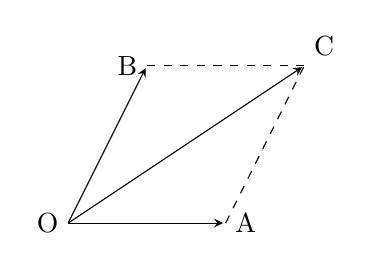
\begin{tikzpicture}
    \draw [->,>=stealth,shorten >=1pt] (0,0)--(2,0) node [anchor=west]{A};
    \draw [->,>=stealth,shorten >=1pt] (0,0)--(1,2) node [anchor=east]{B};
    \draw [dashed] (1,2) --(3,2);
    \draw [dashed] (2,0)--(3,2);
    \draw [->,>=stealth,shorten >=1pt] (0,0)--(3,2) node [anchor=south west]{C};
    \draw (0,0) node [anchor=east]{O};
  \end{tikzpicture}
  \caption{平行四边形定则}
  \label{fig:parallelogram law}
\end{figure}

$$\vec{C}=\vec{A}+\vec{B}$$

数学上舍弃矢量的实际含义,就抽象为数学中的概念---向量.同学们要掌握向量的计算方法,如果不熟悉的话,请参考数学书籍先补充上这一部分知识.

\subsubsection{路程}

路程指\CJKunderwave{物体运动轨迹的长度},是一个\CJKunderwave{标量}.

\subsubsection{位移}

位移指从\CJKunderwave{初位置}到\CJKunderwave{末位置}的有向线段,是一个矢量,大小就是该有向线段的长度,方向就是前头所指的方向.

描述一个物体的机械运动,准确的应该使用位移.但是同学们在读初中的时候使用路程来计算,并没有遇到错误,那是因为在初中研究的都是单向直线运动,\CJKunderwave{单向直线运动中位移的大小与路程相等},同时只有一个方向,所以在计算过程中略去方向的考虑并不会导致问题.

\begin{figure}[H]
  \centering
  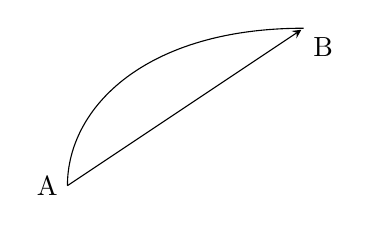
\begin{tikzpicture}
    \draw (0,0) .. controls (0,1) and (1,2) .. (3,2);
    \draw [->,>=stealth,shorten >=1pt] (0,0) -- (3,2);
    \draw (0,0) node [anchor=east]{A};
    \draw (3,2) node [anchor=north west]{B};
  \end{tikzpicture}
  \caption{位移}
  \label{fig:displacement}
\end{figure}

如图\ref{fig:displacement}所示,由A到B的位移记为$\overrightarrow{AB}$,但是路程由两个不同的路径是不同的.同时也能看到,对于\CJKunderwave{曲线运动它的位移大小小于路程},但是单向直线运动中它们是相等的.

对于直线运动的位移可以用$x_1$表示质点的起始位置,$x_2$表示质点的末位置,则以$\Delta x=x_2-x_1$表示位移.
如果$\Delta x>0$表示位移方向向右,如果$\Delta x<0$表示位移方向向左.

\begin{figure}[H]
  \centering
    \begin{tikzpicture}
      \draw [->] (0,0)--(3,0) node [anchor=north] {\small $x/m$};
      \draw (1,0)--(1,4pt) node [anchor=south] {\small $x_1$};
      \draw (2,0)--(2,4pt) node [anchor=south] {\small $x_2$};
    \end{tikzpicture}
  \caption{直线运动的位移}
\end{figure}

  \begin{selection}
    s1.下列关于位移(矢量)和温度(标量)的说法中,正确的是[D]
    A.两个运动物体的位移大小均为$30m$,则这两个位移一定相同
    B.做直线运动的两个物体的位移$x_1=3m$, $x_2=-5m$,则$x_1>x_2$
    C.温度计计数有正也有负,其正,负号表示方向
    D.温度计计数的正负号表示温度的高低,不能表示方向

    a.*

    e.两个矢量相同指矢量的大小和方向两个要素都相同,所以A由于可能方向不同,所以错;直线运动的位移的``$+$''表示与正方向相同,``$-$''表示与正方向相反;温度是标量,标量的正负号表示大小(也就是温度的高低).

    s2.(多选)关于位移和路程,下列说法正确的是[BCD]
    A.在某一段时间内物体运动的位移为零,则该物体一定是静止的
    B.在某一段时间内物体运动的路程为零,则该物体一定是静止的.
    C.在直线运动中,物体的位移大小可能等于其路程
    D.在曲线运动中,物体的位移大小一定小于其路程

    a.BCD

    e.位移为零,表明该物体在运动过程中的初、末位置相同,物体不一定静止,A项错误;路程为零,表明运动轨迹的长度为零,物体一定静止,B项正确;当物体做单向直线运动时,其位移大小等于路程,C项正确;物体在做曲线运动时,初、末位置直线距离小于轨迹长度,所以位移大小一定小于路程,D项正确.

    s3.(多选)对位移和路程理解正确的是[BC]
    A.路程是个标量,是由初始位置指向终止位置的有向线段
    B.位移是个矢量,是由初始位置指向终止位置的有向线段
    C.路程是物体实际运动轨迹的长度,它没有方向
    D.当物体做直线运动时,位移和路程是相同的物理量

    a.BC

    e.路程是物体实际运动轨迹的长度,是标量;位移是由初始位置指向终止位置的有向线段,是矢量.当物体做单向直线运动时,两者大小相等,但不相同.综上,选项B,C正确.

  \end{selection}
  \begin{calculate}
   c1.如
   <:
   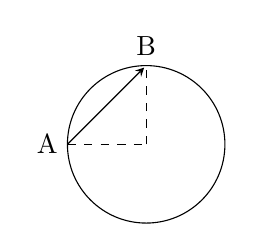
\begin{tikzpicture}
     \draw (0,0) circle [radius=1];
     \draw [->,>=stealth,shorten >=1pt] (-1,0) --(0,1);
     \draw (-1,0) node [anchor=east]{A};
     \draw (0,1) node [anchor=south]{B};
     \draw [dashed] (0,0) --(0,1);
     \draw [dashed] (-1,0)--(0,0);
   \end{tikzpicture}
   :>
   所示,一质点沿半径为$20cm$ 的圆周自A 点出发,逆时针运动$\cfrac{3}{4}$圆周到达B点.求质点的位移和路程.

a. 位移大小为$28.3cm$,方向自A点指向B点,路程为$94.2cm$

e.如图,位移大小为AB线段的长度
$$AB=\sqrt{2}r\approx28.3cm$$
方向:由A点指向B点
\newline
路程为
$$s=\cfrac{3}{4}\cdot2\pi r=94.2cm$$

c2.一个袋子里有$40kg$ 大米,再放入$30kg$大米,袋子中大米的质量是多少?如果一位同学从操场中心A点出发向北走了$40m$ 到达B点,然后又向西走了$30m$ 到达C点,则他从A点到C点的路程是多大?位移是多少?从大小的计算方法上看,质量、路程和位移有什么不同?

a.见解析

e.袋子中大米的质量是$40kg+30kg=70kg$.如
<:
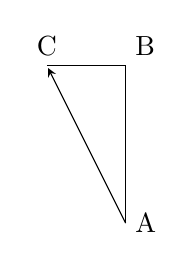
\begin{tikzpicture}
  \draw [->,>=stealth,shorten >=1pt] (0,0)--(-1,2) node [anchor=south]{C};
  \draw (0,0) -- (0,2) node [anchor=south west]{B};
  \draw (-1,2)--(0,2);
  \draw (0,0) node [anchor=west]{A};
\end{tikzpicture}
:>所示,路程是$40m+30m=70m$,位移从A点指向C点的有向线段,大小为$AC=50m$.质量,路程是标量,遵从算术加减法的法则,可以直接相加减;位移是矢量,不能直接相加减,位移的大小等于初位置指向末位置的有向线段的长度.

  \end{calculate}

